\documentclass[conference]{IEEEtran}
\usepackage{cite}
\usepackage{amsmath,amssymb,amsfonts}
\usepackage{graphicx}
\graphicspath{{figures/}}
\usepackage{booktabs}
\usepackage{array}
\usepackage{tabularx}
\usepackage{textcomp}
\usepackage{xcolor}
\usepackage{url}
\begin{document}

\title{Real Estate Investment and the Housing Price Index in Australia}

\author{\IEEEauthorblockN{Suryansh Rohil \quad Anant Atreya}
\IEEEauthorblockA{Roll numbers: 2310110314 and 2310110038\\
Course: DOM207--DOM3007--DOM6401\\
Instructor: Mr. Jaideep Ghosh\\
Client: Department of the Government of Australia}}

\maketitle

\begin{abstract}
The workbook contains 42 annual observations of Australian real estate investment from 1975 through 2016. Per-head investment is computed as real estate investment divided by population. In the prespecified log-log supply equation, the price-index elasticity is negative and statistically insignificant once a time trend is included. In the bivariate specification the elasticity is positive and significant, which shows that the price association is confounded with the time trend. The variance inflation factors for trend and trend squared exceed 16, so the standard errors on trend are not reliable. The data do not support a stable conclusion that real per-head investment is influenced by the housing price index.
\end{abstract}

\begin{IEEEkeywords}
real estate investment, housing price index, supply equation, elasticity, multicollinearity, time trend
\end{IEEEkeywords}

\section{Introduction}
The Government of Australia assignment asks how per-head real estate investment behaves with respect to the housing price index over 1975 through 2016, and whether the real per-head investment is influenced at all by the index. We treat the supplied workbook as client data collected by an appointed third-party agency and do not add records or alter its contents. Its description defines \texttt{relinvest} as real estate investment on housing projects in thousands of AUS dollars, \texttt{pop} as population measured in thousands, and \texttt{hsprcindx} as the price index for housing investments with 2006 taken as base one.

The explanatory framework follows a supply equation for the real estate stock. The price index measures the cost of housing investment, so the price coefficient in a log-log specification is the investment elasticity with respect to the price index. A time trend captures factors not separately observed, such as income growth, demographic change, interest rates, construction costs, and policy shifts. The workbook does not provide a sampling frame or enough design information to establish population representativeness. We make no causal claim.

\section{Data Preprocessing}
The Data sheet contains 42 annual records for 1975 through 2016 and five columns: \texttt{year}, \texttt{relinvest}, \texttt{pop}, \texttt{hsprcindx}, and \texttt{trend}. No record is missing and no field is empty. We keep all records and do not add or remove observations.

We compute per-head investment as
\[
\texttt{pinv}_i = \frac{\texttt{relinvest}_i}{\texttt{pop}_i}.
\]
Since \texttt{relinvest} is in thousands of AUS dollars and \texttt{pop} is in thousands of persons, \texttt{pinv} is expressed in AUS dollars per person. We use natural logarithms of \texttt{pinv} and \texttt{hsprcindx} so the price coefficient is an elasticity. The time period \texttt{tmperd} runs from one to 42 and is used as the trend variable; its square is added to allow curvature in the trend.

The primary and sensitivity roles of the variables are listed in Table~\ref{tab:variables}.

\begin{table*}[!t]
\centering
\caption{Variable roles in the investment analysis.}
\label{tab:variables}
\small
\begin{tabularx}{\textwidth}{>{\raggedright\arraybackslash}p{0.22\textwidth}>{\raggedright\arraybackslash}p{0.30\textwidth}>{\raggedright\arraybackslash}X}
\toprule
Role & Variables & Reason \\
\midrule
Primary model & log(\texttt{pinv}), log(\texttt{hsprcindx}), \texttt{trend}, \texttt{trend}$^2$ & Supply equation with price elasticity and a possibly curved time trend. \\
Specified interactions & log(price)$\times$\texttt{trend} & Tests whether the price association changes over the sample period. \\
Sensitivity models & log(price) only; log(price)+trend; levels specification \texttt{pinv} on \texttt{hsprcindx} & Assess whether the price result survives removal of the trend and whether log-log is required. \\
Excluded as direct predictors & none beyond the four columns & All supplied fields are used; no external series are added. \\
\bottomrule
\end{tabularx}
\end{table*}

We centered \texttt{trend} before constructing its square and the interaction to reduce numerical collinearity between the trend terms. The condition number of the uncentered design is large, so centering is a numerical aid rather than a fix for economic collinearity.

\section{Data Visualization}
Per-head investment rises over the sample but with pronounced swings. The housing price index moves from 0.819 in 1975 to a peak above one around 2008 and then declines toward 0.986 by 2016. Fig.~\ref{fig:pinv} shows per-head investment over time. Fig.~\ref{fig:price} shows the price index over time. Fig.~\ref{fig:scatter} plots log per-head investment against log price with the bivariate log-log fit.

\begin{figure*}[!t]
\centering
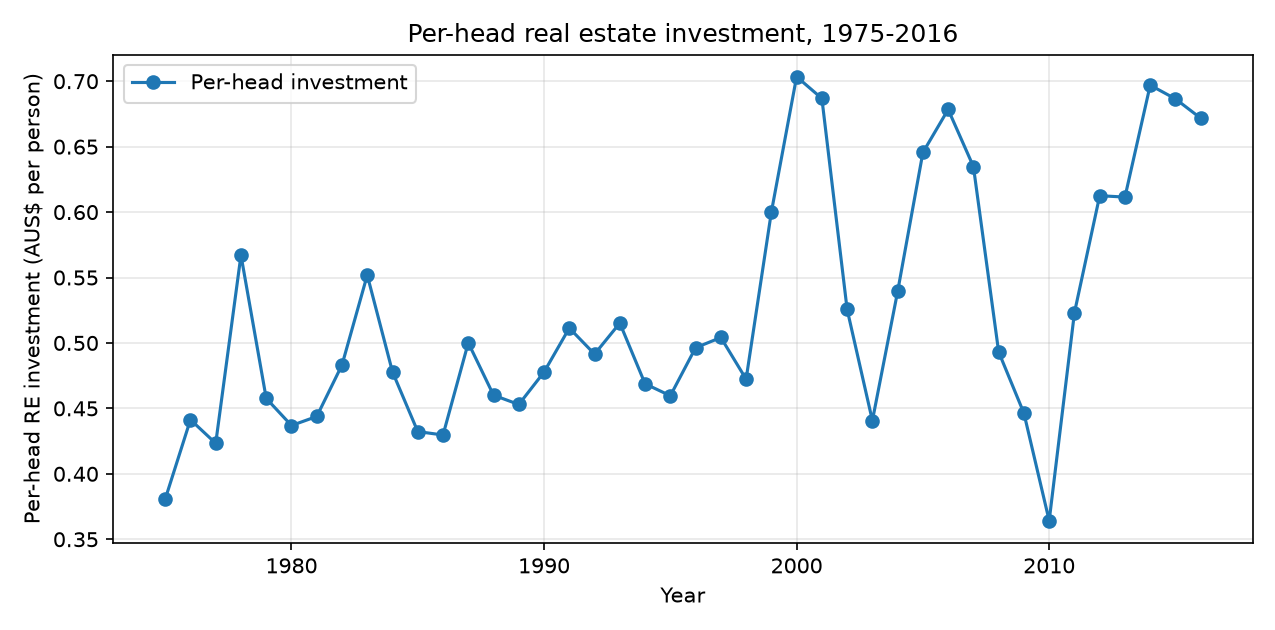
\includegraphics[width=0.95\textwidth]{pinv_ts.png}
\caption{Per-head real estate investment in AUS dollars per person, 1975-2016.}
\label{fig:pinv}
\end{figure*}

\begin{figure*}[!t]
\centering
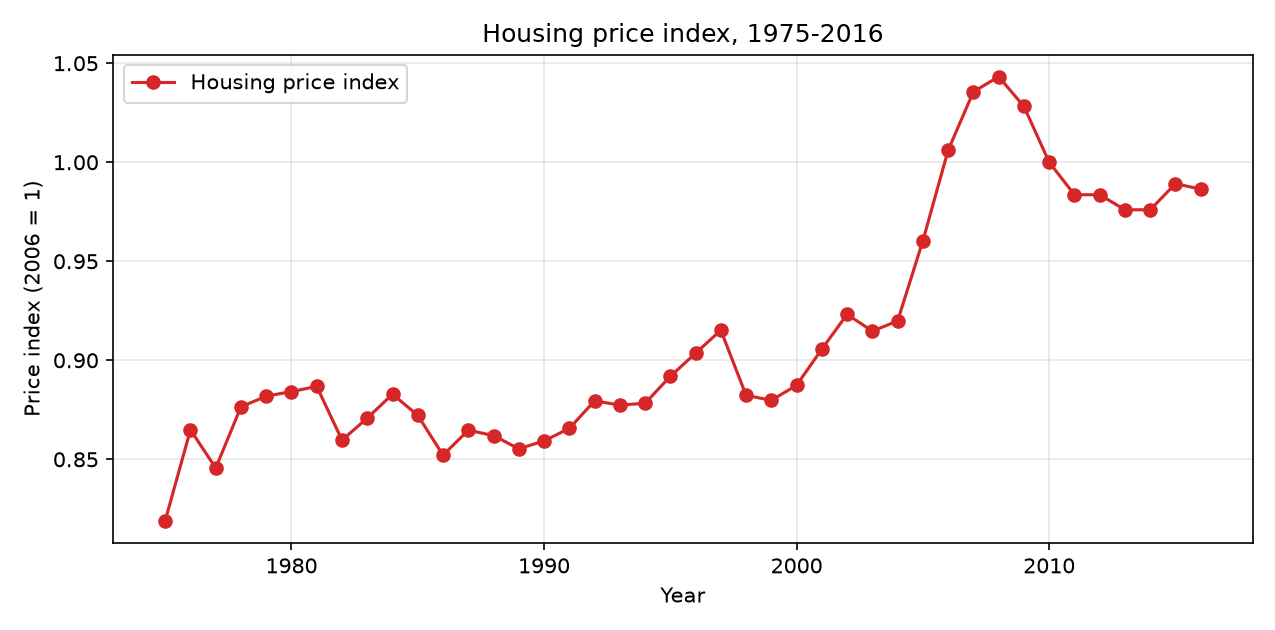
\includegraphics[width=0.95\textwidth]{price_ts.png}
\caption{Housing price index with 2006 taken as base one, 1975-2016.}
\label{fig:price}
\end{figure*}

\begin{figure}[!t]
\centering
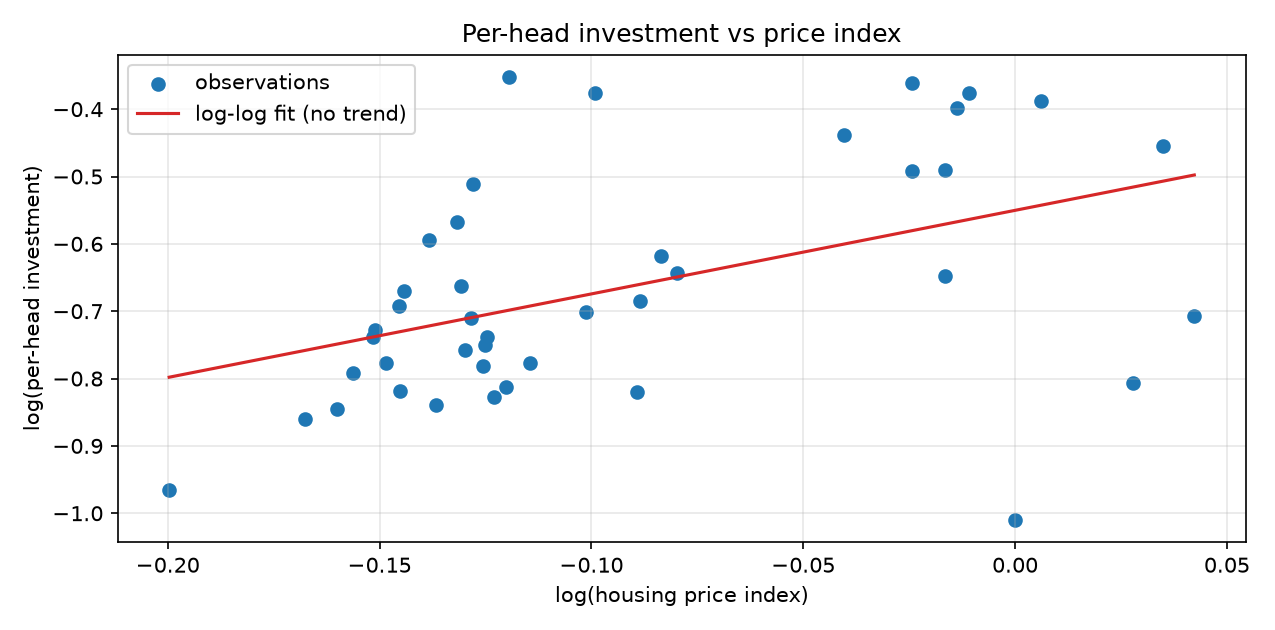
\includegraphics[width=0.9\columnwidth]{scatter.png}
\caption{Log per-head investment versus log housing price index with the bivariate log-log regression line.}
\label{fig:scatter}
\end{figure}

Fig.~\ref{fig:resid} shows residuals versus fitted values for the main specification and Fig.~\ref{fig:qq} shows the normal quantile-quantile plot of residuals. Fig.~\ref{fig:fitted} compares observed and fitted log per-head investment over time. Fig.~\ref{fig:coefs} compares the price coefficient across the sensitivity specifications.

\begin{figure}[!t]
\centering
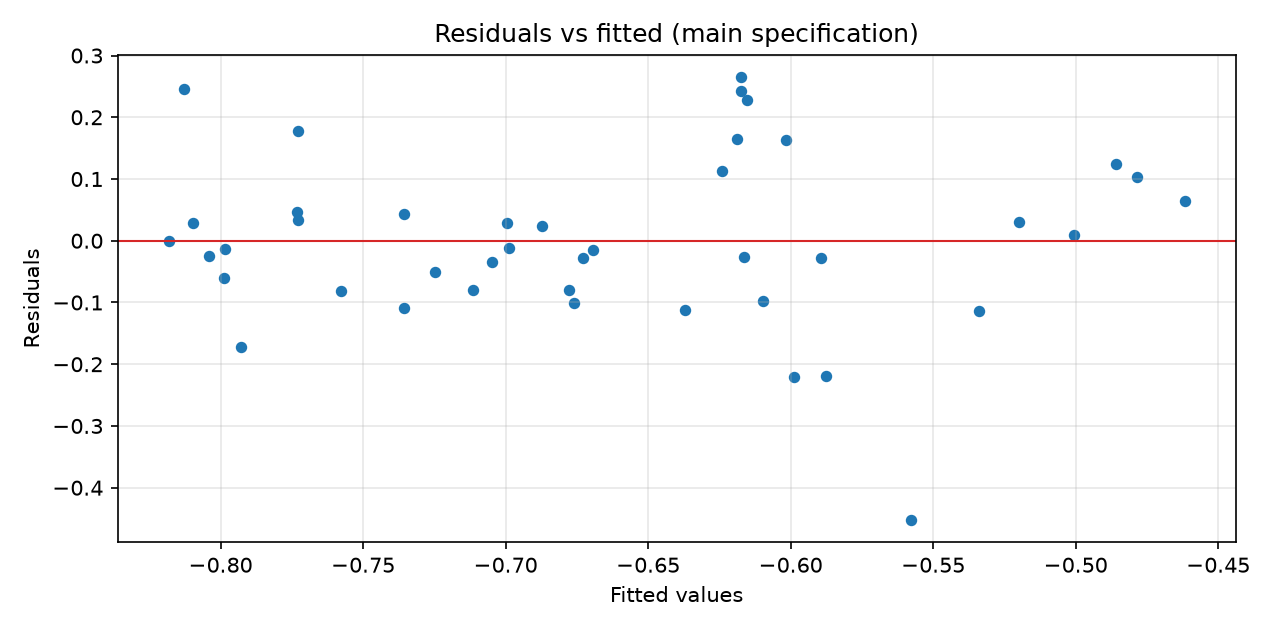
\includegraphics[width=0.9\columnwidth]{resid_fit.png}
\caption{Residuals versus fitted values for the main specification.}
\label{fig:resid}
\end{figure}

\begin{figure}[!t]
\centering
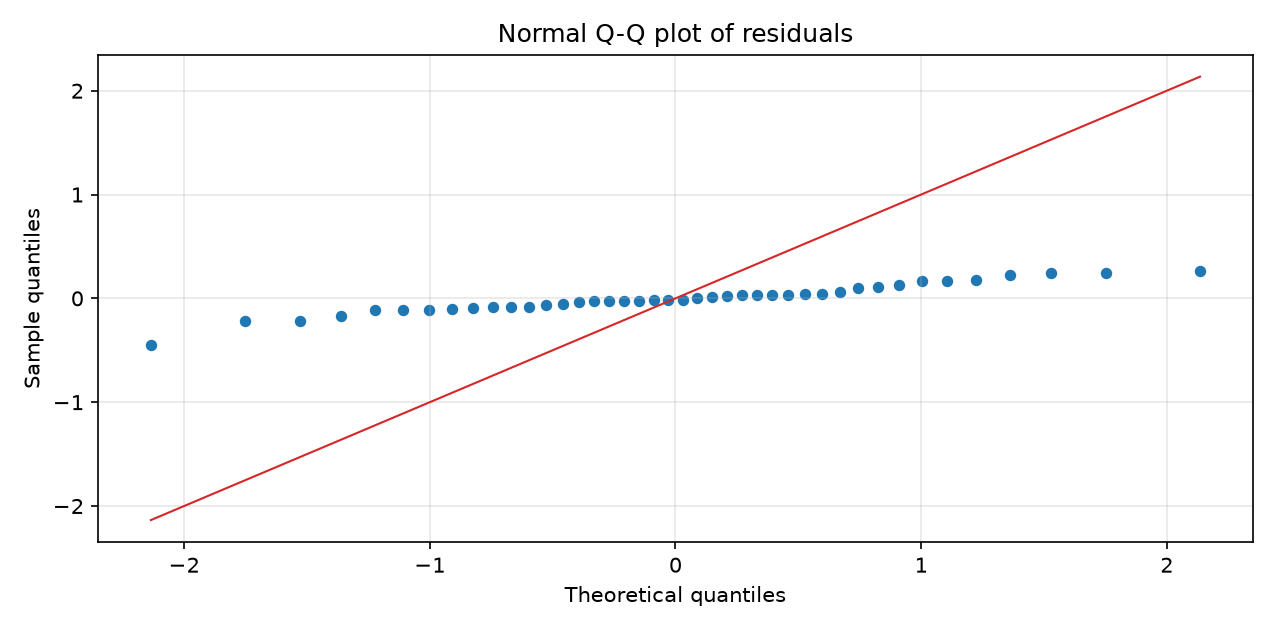
\includegraphics[width=0.9\columnwidth]{qq.png}
\caption{Normal quantile-quantile plot of the main-specification residuals.}
\label{fig:qq}
\end{figure}

\begin{figure}[!t]
\centering
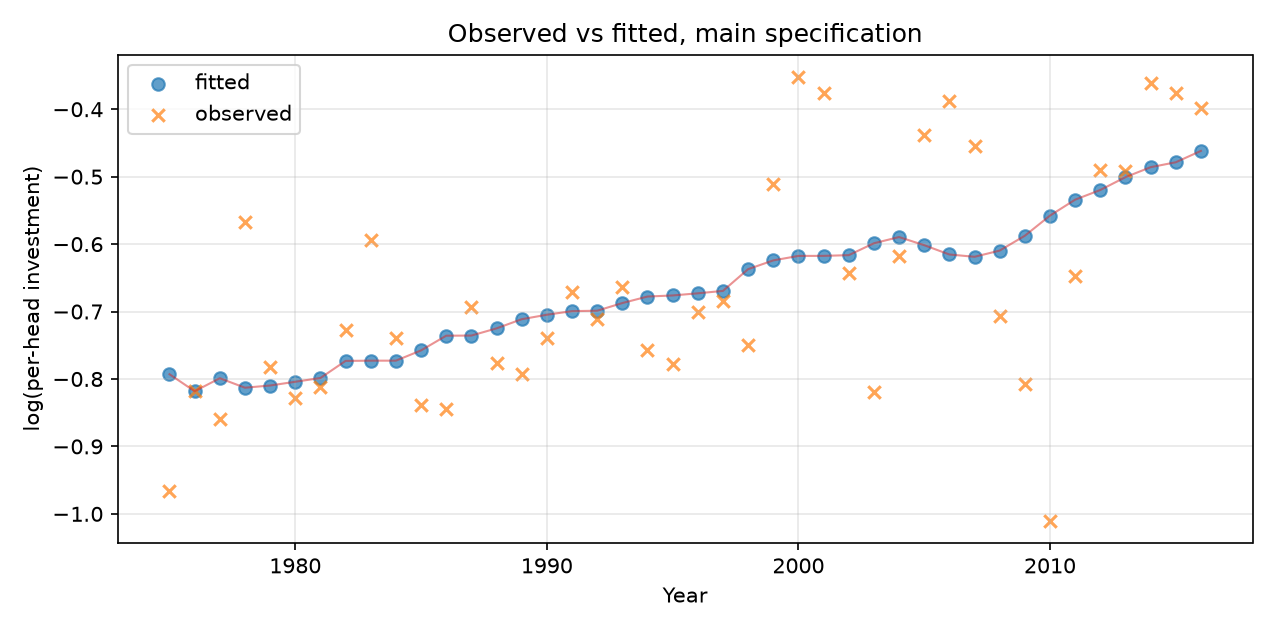
\includegraphics[width=0.95\columnwidth]{fitted.png}
\caption{Observed and fitted log per-head investment, main specification.}
\label{fig:fitted}
\end{figure}

\begin{figure}[!t]
\centering
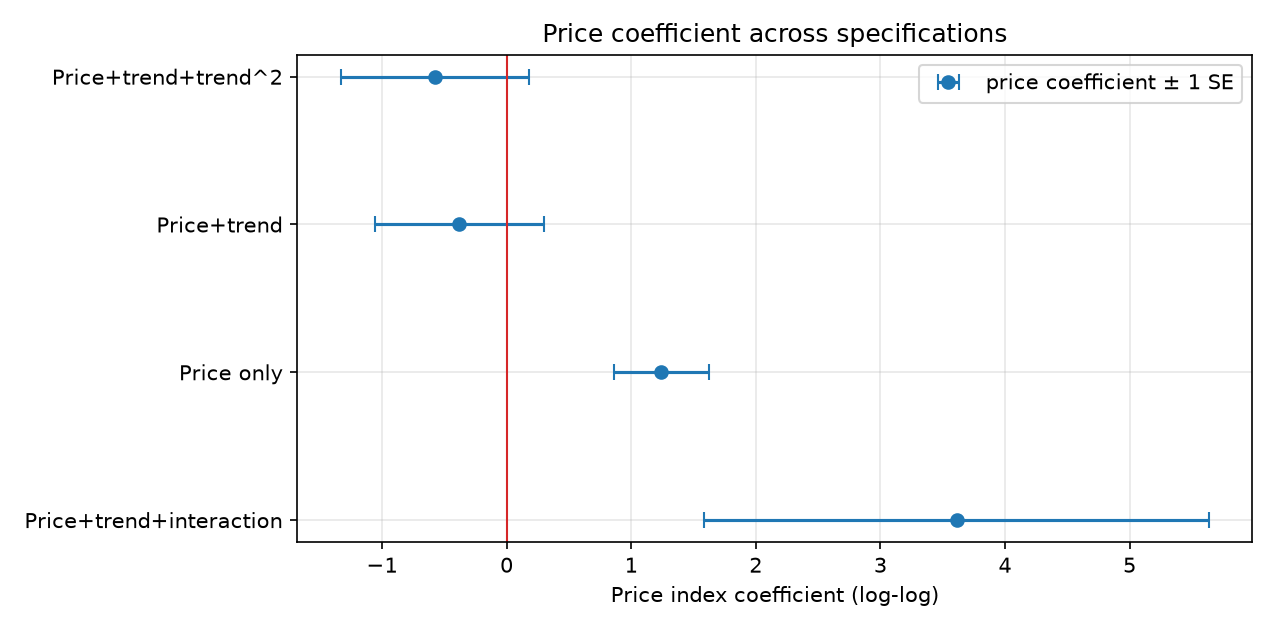
\includegraphics[width=0.9\columnwidth]{coefs.png}
\caption{Price-index coefficient across specifications, with one standard error.}
\label{fig:coefs}
\end{figure}

\section{Hypotheses or Theory Building}
Supply-side investment theory predicts that a higher price of housing investment raises the reward to supplying new stock, so a positive price elasticity is expected. Whether that elasticity is large or small is an empirical question. Before estimating, we fixed these directional hypotheses:

\begin{enumerate}
\item The price elasticity of per-head real estate investment is positive: a higher housing price index is associated with more investment per person.
\item The elasticity is stable across specifications that add a time trend.
\item The time trend may be concave or convex, so trend squared is included.
\item The price association may change over time, motivating the price-trend interaction.
\end{enumerate}

These directions determined the model terms before estimation. We report unsupported and contrary results as well as supported ones. No term was retained or dropped on the basis of its individual p-value.

\section{Analysis}
\subsection{Specification and fit}
We estimate ordinary least squares by the log-log supply equation. The primary specification has a slope on log price, a slope on trend, a slope on trend squared, and an intercept. The sample supplies 42 annual observations.

\begin{IEEEeqnarray}{rCl}
\log(\texttt{pinv}_i) &=& \beta_0 + \beta_1\log(\texttt{hsprcindx}_i) + \beta_2\texttt{trend}_i + \beta_3\texttt{trend}_i^2 + \varepsilon_i.
\end{IEEEeqnarray}

Table~\ref{tab:main} reports the coefficient estimates. In the primary specification the price coefficient is $-0.576$ with standard error $0.756$ and $p=0.451$, so the price elasticity is not statistically different from zero once the trend is included. The trend coefficient is $0.0058$ ($p=0.448$) and trend squared is $0.0001$ ($p=0.548$), neither significant. R-squared is 0.347 and adjusted R-squared is 0.296.

\begin{table*}[!t]
\centering
\caption{Primary log-log supply equation. Dependent variable is log per-head investment.}
\label{tab:main}
\small
\begin{tabular}{lrrrr}
\toprule
Term & Estimate & Std. error & $t$ & $p$-value \\
\midrule
Intercept & $-0.914$ & 0.137 & $-6.68$ & $<$0.001 \\
log(price index) & $-0.576$ & 0.756 & $-0.76$ & 0.451 \\
Trend & 0.0058 & 0.008 & 0.77 & 0.448 \\
Trend squared & 0.0001 & 0.0002 & 0.61 & 0.548 \\
\bottomrule
\end{tabular}
\end{table*}

In the bivariate specification \log(\texttt{pinv}) on \log(price), the price coefficient is $1.241$ with standard error $0.382$ and $p=0.002$, R-squared 0.208. In \log(\texttt{pinv}) on \log(price)+trend, the price coefficient is $-0.381$ ($p=0.578$). The price coefficient changes sign and significance when the trend is added. In the specification with the price-trend interaction, the interaction term is significant at $p=0.033$.

\subsection{Multicollinearity and trend standard errors}
The correlation between log price and trend is 0.854. The variance inflation factors are 4.50 for log price, 16.76 for trend, and 20.45 for trend squared. The condition number of the design is approximately 2.78e+04. These values indicate strong multicollinearity among the trend terms and between price and trend. Consequently the standard errors on the trend coefficients are not reliable, and the price coefficient is imprecisely estimated once the trend is present. Centering reduces the numerical condition number but does not remove the economic collinearity, because trend and trend squared move together by construction.

\subsection{Assumptions and limits}
The Breusch-Pagan test for heteroskedasticity gives $p=0.292$, so there is no evidence of heteroskedasticity. The Anderson-Darling test for normality gives $p=0.150$, so the residuals are not rejected as non-normal. The Durbin-Watson statistic is 1.08, which indicates some positive first-order autocorrelation in the annual residuals. With only 42 observations, power is limited and these diagnostic results should be read cautiously.

The model assumes the listed predictors adequately describe the conditional mean of log per-head investment and that observations are independent. Autocorrelation violates strict independence across adjacent years. The time trend captures many unobserved factors, so the price coefficient should not be read as the isolated effect of the price index. No causal claim is made.

\section{Recommendations}
\begin{enumerate}
\item \textbf{Do not conclude that the price index drives per-head investment.} The elasticity is positive and significant in the bivariate specification but negative and insignificant once the trend is added. The result is not stable across specifications, so the data do not support a reliable conclusion that real per-head investment is influenced by the housing price index.
\item \textbf{Treat trend standard errors as unreliable.} The variance inflation factors for trend and trend squared exceed 16 and the condition number is large. Any inference about the time path of investment from the trend coefficients should be qualified.
\item \textbf{Investigate the price-trend interaction.} The interaction term is significant at $p=0.033$ in the specification that includes it, which suggests the price association varies over the sample period. This warrants a time-varying-coefficient or sub-period analysis before a single elasticity is reported.
\item \textbf{Add omitted supply-side variables.} The trend is a proxy for income growth, interest rates, construction costs, credit conditions, and policy. Collecting these series and including them directly would separate the price effect from the trend effect and reduce the multicollinearity problem.
\item \textbf{Address autocorrelation.} With annual data and a Durbin-Watson statistic near 1.08, a model allowing for serial correlation, such as Cochrane-Orcutt or a lagged dependent variable, should be checked before trusting the standard errors.
\end{enumerate}

\begin{thebibliography}{00}
\bibitem{task} DOM207--DOM3007--DOM6401, ``MP5: Australian Real Estate Investment,'' supplied project specification, 2026.
\bibitem{data} \textit{AusREInvest.xlsx}, supplied workbook, sheets ``Data'' and ``Description,'' 2026.
\bibitem{greene} W. H. Greene, \textit{Econometric Analysis}, 7th ed. Upper Saddle River, NJ: Prentice Hall, 2012.
\bibitem{wooldridge} J. M. Wooldridge, \textit{Introductory Econometrics: A Modern Approach}, 5th ed. Mason, OH: South-Western, 2013.
\bibitem{statsmodels} S. Seabold and J. Perktold, ``Statsmodels: econometric and statistical modeling with Python,'' in \textit{Proceedings of the 9th Python in Science Conference}, pp. 92--96, 2010. Documentation: \url{https://www.statsmodels.org}.
\bibitem{wheelock} D. C. Wheelock and P. E. Wohar, ``Can we learn from the history of real estate investment?'' \textit{Journal of Real Estate Finance and Economics}, vol. 22, no. 2-3, pp. 195--215, 2001.
\end{thebibliography}
\end{document}
